%%%%%%%%%%%%%%%%%%%%%%%%%%%%%%%%%%%%%%%%%
% Oliver Lemon made minor edits (jan 2015)  to : 
% Masters/Doctoral Thesis 
% LaTeX Template
% Version 1.43 (17/5/14)
%
% This template has been downloaded from:
% http://www.LaTeXTemplates.com
%
% Original authors:
% Steven Gunn 
% http://users.ecs.soton.ac.uk/srg/softwaretools/document/templates/
% and
% Sunil Patel
% http://www.sunilpatel.co.uk/thesis-template/
%
% License:
% CC BY-NC-SA 3.0 (http://creativecommons.org/licenses/by-nc-sa/3.0/)
%
% Note:
% Make sure to edit document variables in the Thesis.cls file
%
%%%%%%%%%%%%%%%%%%%%%%%%%%%%%%%%%%%%%%%%%

%----------------------------------------------------------------------------------------
%	PACKAGES AND OTHER DOCUMENT CONFIGURATIONS
%----------------------------------------------------------------------------------------

\documentclass[12pt, oneside]{Thesis} % The default font size and one-sided printing (no margin offsets)

\graphicspath{{Pictures/}} % Specifies the directory where pictures are stored

\usepackage[en-GB]{datetime2}

\usepackage{multirow}

\newcommand*\rot{\rotatebox{90}}

%paragraph indentation
\setlength{\parindent}{3em} 

\setcounter{tocdepth}{1}

\usepackage[square, sort&compress]{natbib} % Use the natbib reference package - read up on this to edit the reference style; if you want text (e.g. Smith et al., 2012) for the in-text references (instead of numbers), remove 'numbers' 
\hypersetup{urlcolor=blue, colorlinks=true} % Colors hyperlinks in blue - change to black if annoying
\renewcommand\bibname{References}

\expandafter\def\expandafter\UrlBreaks\expandafter{\UrlBreaks%  save the current one
	\do\a\do\b\do\c\do\d\do\e\do\f\do\g\do\h\do\i\do\j%
	\do\k\do\l\do\m\do\n\do\o\do\p\do\q\do\r\do\s\do\t%
	\do\u\do\v\do\w\do\x\do\y\do\z\do\A\do\B\do\C\do\D%
	\do\E\do\F\do\G\do\H\do\I\do\J\do\K\do\L\do\M\do\N%
	\do\O\do\P\do\Q\do\R\do\S\do\T\do\U\do\V\do\W\do\X%
	\do\Y\do\Z}

\usepackage[final]{pdfpages}
\usepackage{eso-pic}
\usepackage{atbegshi}
\usepackage{pdflscape}

\usepackage{wrapfig}

%\newcommand{\specialcell}[2][c]{%
%	\begin{tabular}[#1]{@{}c@{}}#2\end{tabular}}

\newcommand{\specialcell}[3][c]{% 		
	\begin{tabular}[#1]{@{}#2@{}}#3\end{tabular}}%

\usepackage{dirtytalk}

\usepackage{verbatim}

\usepackage{float}
%\usepackage[demo]{graphicx}
%\usepackage{caption}
\usepackage{subcaption}

\usepackage{tikz}
\def\checkmark{\tikz\fill[scale=0.4](0,.35) -- (.25,0) -- (1,.7) -- (.25,.15) -- cycle;} 

\usepackage{soul}
\newcommand{\hlc}[2][pink]{ {\sethlcolor{#1} \hl{#2}}}

\usepackage[document]{ragged2e}
\hyphenchar\font=-1 %to remove all hyphenation
\sloppy %To get rid of overfull boxes

\usepackage{cleveref}


\begin{document}

\frontmatter % Use roman page numbering style (i, ii, iii, iv...) for the pre-content pages

\setstretch{1.3} % Line spacing of 1.3

% Define the page headers using the FancyHdr package and set up for one-sided printing
\fancyhead{} % Clears all page headers and footers
\rhead{\thepage} % Sets the right side header to show the page number
\lhead{} % Clears the left side page header

\pagestyle{fancy} % Finally, use the "fancy" page style to implement the FancyHdr headers

\newcommand{\HRule}{\rule{\linewidth}{0.5mm}} % New command to make the lines in the title page

% PDF meta-data
\hypersetup{pdftitle={\ttitle}}
\hypersetup{pdfsubject=\subjectname}
\hypersetup{pdfauthor=\authornames}
\hypersetup{pdfkeywords=\keywordnames}

%----------------------------------------------------------------------------------------
%	TITLE PAGE
%----------------------------------------------------------------------------------------

\begin{titlepage}
\begin{center}

\textsc{\LARGE \univname}\\[1.5cm] % University name
%\textsc{\Large Masters Thesis}\\[0.5cm] % Thesis type

\HRule \\[0.4cm] % Horizontal line
{\LARGE \bfseries {D11PJ Industrial Project}}\\[0.4cm] % Thesis title
\HRule \\[1.5cm] % Horizontal line
 
\vfill
 
H00165151
\\ \authornames % Author name - remove the \href bracket to remove the link
 
\large \textit{\degreename}\\[0.3cm] % University requirement text

\deptname\\[1cm] % Research group name and department name
 
{\large \DTMlangsetup{showdayofmonth=false} \today}\\[1cm] % Date
\includegraphics[width=4.5cm]{./figures/HWlogo2016.jpg} % University/department logo - uncomment to place it
 
\vfill
\end{center}

\end{titlepage}


%----------------------------------------------------------------------------------------
%	ABSTRACT PAGE
%----------------------------------------------------------------------------------------

\addtotoc{Abstract} % Add the "Abstract" page entry to the Contents

%\abstract{\addtocontents{toc}{\vspace{1em}} % Add a gap in the Contents, for aesthetics

\input{Front_Matter/02-Abstract.tex}

\clearpage % Start a new page


%----------------------------------------------------------------------------------------
%	LIST OF CONTENTS/FIGURES/TABLES PAGES
%----------------------------------------------------------------------------------------

\pagestyle{fancy} % The page style headers have been "empty" all this time, now use the "fancy" headers as defined before to bring them back

\lhead{\emph{Contents}} % Set the left side page header to "Contents"
\tableofcontents % Write out the Table of Contents

\lhead{\emph{List of Figures}} % Set the left side page header to "List of Figures"
\listoffigures % Write out the List of Figures

\lhead{\emph{List of Tables}} % Set the left side page header to "List of Tables"
\listoftables % Write out the List of Tables

%----------------------------------------------------------------------------------------
%	ABBREVIATIONS
%----------------------------------------------------------------------------------------

\clearpage % Start a new page

\setstretch{1.5} % Set the line spacing to 1.5, this makes the following tables easier to read

\lhead{\emph{Abbreviations}} % Set the left side page header to "Abbreviations"
\listofsymbols{ll} % Include a list of Abbreviations (a table of two columns)
{
\textbf{AE} & \textbf{A}rchitectural \textbf{E}ngineering \\
%
\textbf{BIM} & \textbf{B}uilding \textbf{I}nformation \textbf{M}odelling \\
%
\textbf{CAD} & \textbf{C}omputer-\textbf{A}ided \textbf{D}esign \\
%
\textbf{CFD} & \textbf{C}omputational \textbf{F}luid \textbf{D}ynamics \\
%
\textbf{DSM} & \textbf{D}emand \textbf{S}ide \textbf{M}anagement \\
%
\textbf{H\&S} & \textbf{H}ealth \textbf{and S}afety \\
%
\textbf{IES} & (See IES-VE) \\
%
\textbf{IES-VE} & \textbf{I}ntegrated \textbf{E}nvironmental \textbf{S}olutions - \textbf{V}irtual \textbf{E}nvironment \\ & (sometimes solely referred to as IES) \\
%
\textbf{iSBEM} & An \textbf{i}nterface for \textbf{S}implified \textbf{B}uilding \textbf{E}nergy \textbf{M}odel \\
%
\textbf{M\&E} & \textbf{M}echanical \textbf{and E}lectrical \\
%
\textbf{POE} & \textbf{P}ost-\textbf{O}ccupancy \textbf{E}valuation \\
%
\textbf{PV} & \textbf{P}hoto\textbf{v}oltaic \\
%
\textbf{RIBA} & \textbf{R}oyal \textbf{I}nstitute of \textbf{B}ritish \textbf{A}rchitects \\
%
\textbf{SAP} & \textbf{S}tandard \textbf{A}ssessment \textbf{P}rocedure \\
%
}


%----------------------------------------------------------------------------------------
%	THESIS CONTENT - CHAPTERS
%----------------------------------------------------------------------------------------

\mainmatter % Begin numeric (1,2,3...) page numbering

\pagestyle{fancy} % Return the page headers back to the "fancy" style

% Include the chapters of the thesis as separate files from the Chapters folder
% Uncomment the lines as you write the chapters

\chapter{Introduction} % Main chapter title

\label{Chapter1} % Change X to a consecutive number; for referencing this chapter elsewhere, use \ref{ChapterX}

\lhead{Chapter 1. \emph{Introduction}} % Change X to a consecutive number; this is for the header on each page - perhaps a shortened title


\chapter{Work Experience} % Main chapter title

\label{Chapter2} % Change X to a consecutive number; for referencing this chapter elsewhere, use \ref{ChapterX}

\lhead{Chapter 2. \emph{Work Experience}} % Change X to a consecutive number; this is for the header on each page - perhaps a shortened title

I have had a total of six work placements since the start of my gap year.
Figure \ref{timeline} provides a timeline of the companies I have worked at.
The focus of this chapter will be on my placement at Sunamp, which was specifically done as part of D11PJ \textit{Industrial Project}.
After describing my experience at Sunamp, I will briefly describe my other work experiences.

\begin{figure}[htbp]
	\centering
	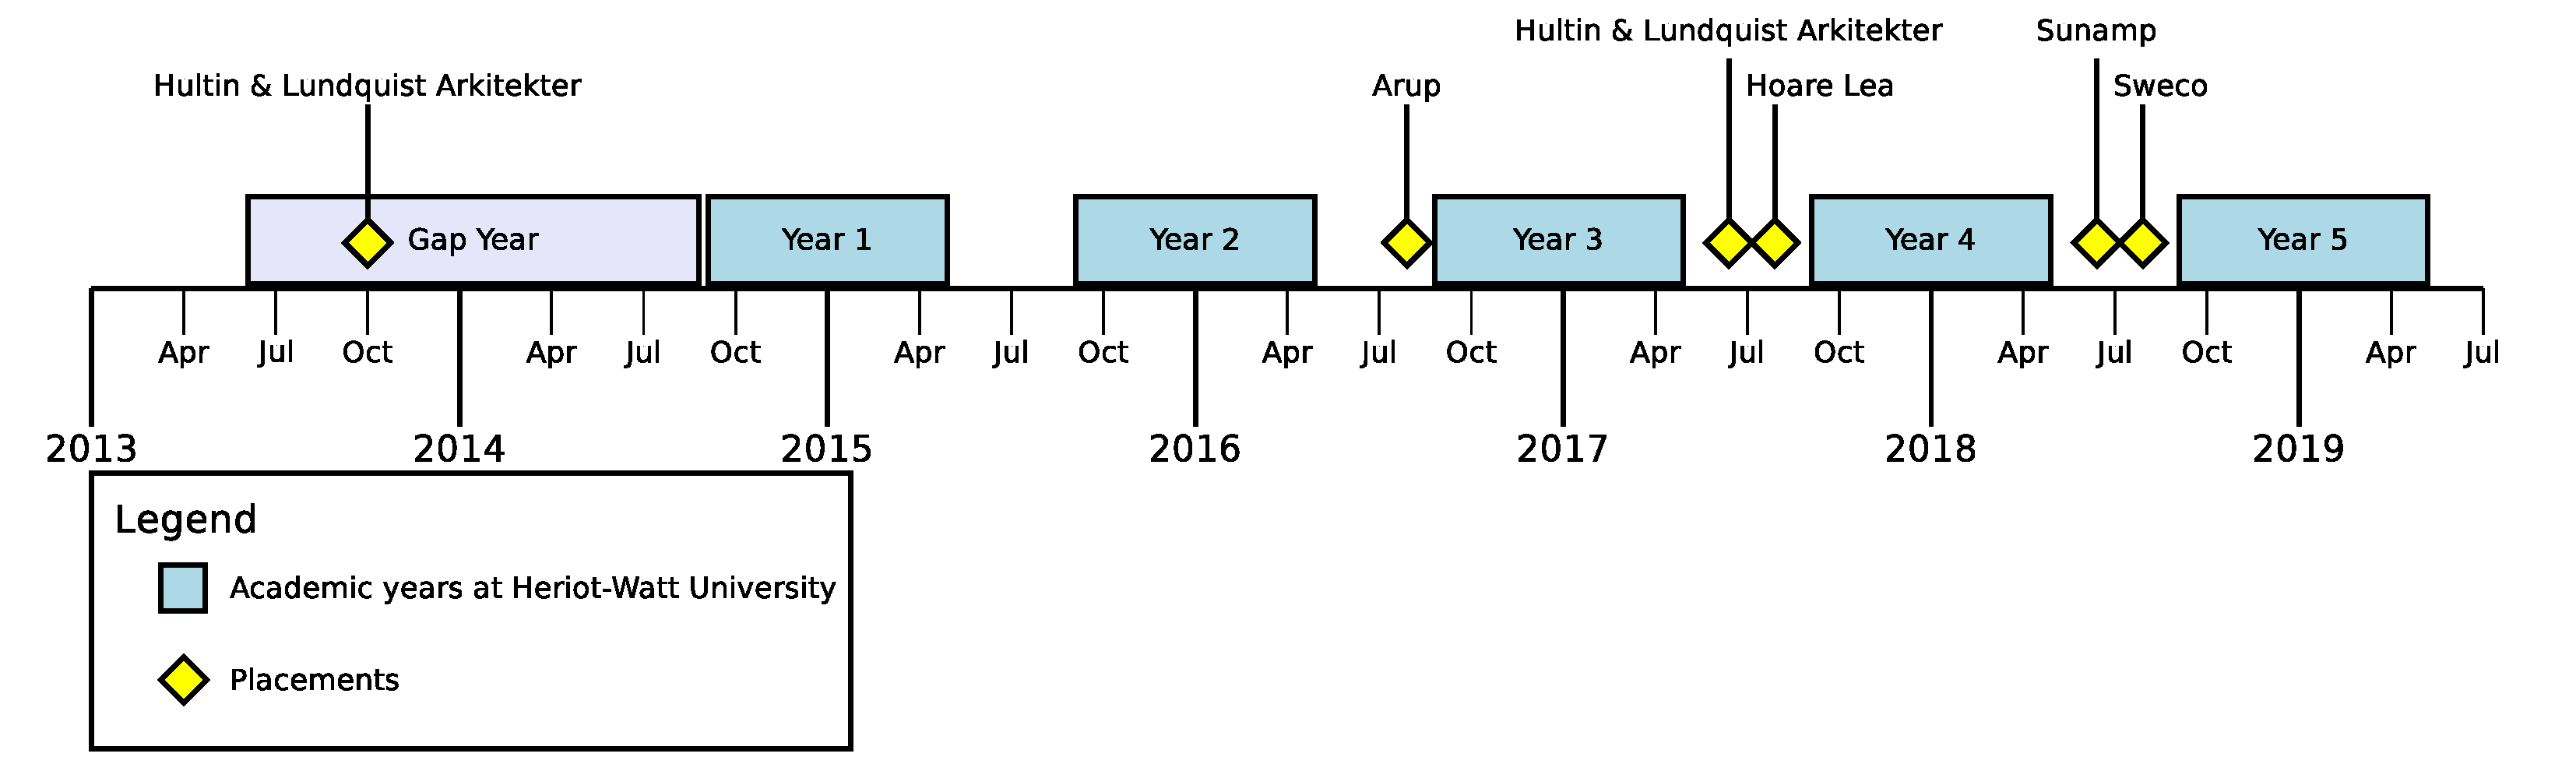
\includegraphics[width=\textwidth]{figures/IP-Timeline.eps}
	\rule{\textwidth}{0.5pt} % use line???
	\caption{Timeline of my work placements since my pre-university gap year.}
	\label{timeline}
\end{figure}


%----------------------------------------------------------------------------------------
%	SECTION 1
%----------------------------------------------------------------------------------------

\section{Sunamp, July - August 2018}

My placement at Sunamp started on 3\textsuperscript{rd} July 2018 and ended on 10\textsuperscript{th} August 2018.
I worked a total of 198 hours there (\hl{see time/ work log in Appendix ...}).


\subsection{Application Process}

I learned about the opportunity of two paid placements with immediate start at Sunamp through David Campbell, the D11PJ course leader.
He had asked applicants for this placement to send him 100 words broadly describing their strengths and preferences, which he would then forward to Sunamp.
A coursemate named Hamish and I were both interested in this opportunity.
\hl{My hundred-word application went as follows:}

Strengths:
\begin{itemize}
	\item I am very familiar with the BIM process, having written a dissertation on collaboration with regards to BIM.
	\item I have work experience in mechanical and electrical consulting engineering.
	\item Organised, flexible, independent and cooperative.
\end{itemize}
Skills:
\begin{itemize}
	\item Advanced skills in Microsoft Office packages and Bluebeam Revu.
	\item Intermediate skills in LaTeX.
	\item Basic modelling skills in Revit, AutoCAD and IES-VE.
	\item Fluent in three languages (English, Swedish and French) with basic knowledge of Spanish.
\end{itemize}
Preferences/ interests:
\begin{itemize}
	\item Highly interested in learning about your application of Phase Change Materials in thermal storage batteries.
	\item Also interested in working with BIM and learning Bentley’s Hevacomp software packages.
\end{itemize}

After the applications, David introduced us applicants to Susan Lang-Bissell, the Managing Director (MD) of Sunamp, via email.
David had asked us to liaise with Susan to arrange a meeting.
To do this, Hamish and I first established our availabilities in the upcoming days.
I then volunteered to liaise with Susan via email on our behalf to find a suitable date and time.

\hl{Try to be more reflective, and less descriptive.
Maybe record (vocally) the story, and then reflect on it out loud. THEN write about it.} 
\chapter{Skills Analysis} % Main chapter title

\label{Chapter3} % Change X to a consecutive number; for referencing this chapter elsewhere, use \ref{ChapterX}

\lhead{Chapter 3. \emph{Skills Analysis}} % Change X to a consecutive number; this is for the header on each page - perhaps a shortened title

In this chapter I analyse, describe and demonstrate the knowledge and skills I have \hl{developed and gained} throughout my university education and work experiences in industry.
This has been done in line with the learning outcomes as stipulated by the Engineering Council for the university programmes it accredits, as well as in line with the Graduate Attributes of Heriot-Watt University.


% Please add the following required packages to your document preamble:
% \usepackage{booktabs}
% \usepackage{multirow}
\begin{table}[]
\caption{The courses I took towards my MEng degree in Architectural Engineering at Heriot-Watt University (include course codes? transpose table!)}
\label{courses}
	\begin{tabular}{@{}lp{8cm}p{7.5cm}@{}}
		\toprule
		& Semester 1 & Semester 2 \\ \midrule
		\multirow{4}{*}{\rot{Year 1}} & \textbullet \hspace{0.5ex}Construction Technology 1 & \textbullet \hspace{0.5ex}Building Services Technology \\
		& \textbullet \hspace{0.5ex}History of the Built Environment & \textbullet \hspace{0.5ex}Mechanics B \\
		& \textbullet \hspace{0.5ex}Introduction to Design & \textbullet \hspace{0.5ex}Introduction to the Environment \\
		& \textbullet \hspace{0.5ex}Mathematics for Engineers and Scientists 1 & \textbullet \hspace{0.5ex}Mathematics for Engineers and Scientists 2 \\ \midrule
		\multirow{4}{*}{\rot{Year 2}} & \textbullet \hspace{0.5ex}Design Project A & \textbullet \hspace{0.5ex}Environment and Behaviour \\
		& \textbullet \hspace{0.5ex}Construction Technology 2 & \textbullet \hspace{0.5ex}Statistics for Science \\
		& \textbullet \hspace{0.5ex}Acoustics and Architectural Design & \textbullet \hspace{0.5ex}Energy Principles and Applications \\
		& \textbullet \hspace{0.5ex}\textit{Hydraulics \& Hydrology A} & \textbullet \hspace{0.5ex}\textit{Design Project B} \\ \midrule
		\multirow{4}{*}{\rot{Year 3}} & \textbullet \hspace{0.5ex}Critical Architectural Studies & \textbullet \hspace{0.5ex}Energy and Buildings \\ 
		& \textbullet \hspace{0.5ex}Procurement and Contracts & \textbullet \hspace{0.5ex}Thermal Performance Studies \\
		& \textbullet \hspace{0.5ex}Design Software Applications & \textbullet \hspace{0.5ex}Design Issues \\
		& \textbullet \hspace{0.5ex}Electrical and Lighting Services for Buildings & \textbullet \hspace{0.5ex}Facilities Management Principles \\ \midrule
		\multirow{4}{*}{\rot{Year 4}} & \textbullet \hspace{0.5ex}Design Project (S1) & \textbullet \hspace{0.5ex}Design Project (S2) \\
		& \textbullet \hspace{0.5ex}Dissertation (S1) & \textbullet \hspace{0.5ex}Dissertation (S2) \\
		& \textbullet \hspace{0.5ex}Laboratory Project & \textbullet \hspace{0.5ex}Sustainable and Intelligent Buildings \\
		& \textbullet \hspace{0.5ex}Inclusive and Safe Environments & \textbullet \hspace{0.5ex}Innovation in Construction Practice \\ \midrule
		\multirow{4}{*}{\rot{Year 5}} & \textbullet \hspace{0.5ex}Industrial Project & \textbullet \hspace{0.5ex}Architectural Acoustics \\
		& \textbullet \hspace{0.5ex}\textit{Water Supply \& Drainage for Buildings} & \textbullet \hspace{0.5ex}Design of Low Carbon Buildings \\
		& \textbullet \hspace{0.5ex}\textit{Climate Change, Sustainability \& Adaptation} & \textbullet \hspace{0.5ex}Thermofluids \\
		&  & \textbullet \hspace{0.5ex}\textit{OPTIONAL} \\ \bottomrule
	\end{tabular}
\end{table}


%----------------------------------------------------------------------------------------
%	SECTION 1
%----------------------------------------------------------------------------------------

\section{Science and Mathematics (SM)}

\subsection*{SM1(i, b, m)}

Multiple courses (mainly from years 2 and 3) have contributed to my knowledge and understanding of scientific principles and methodology necessary to underpin my education in Architectural Engineering.
A main contributor was \textit{Thermal Performance Studies}.
On this course I learned the scientific principles of psychrometrics, i.e. the properties of air-vapour mixtures (especially/ like air), and how to use this knowledge in the design of air conditioners, heat exchangers and cooling towers.
Learning about the environmental effects of refrigerants has contributed to my understanding of the evolution of air conditioners, from using carbon and fluoride based refrigerants to water and eventually phase change materials (PCMs) like Sunamp uses.

Learning the scientific principles of related disciplines have helped me enrich my appreciation of the scientific and engineering context of my discipline.
\textit{Statistics for Science} has, for example, helped me understand the proper methodology behind sampling populations and to identify when bias in data.
\textit{Hydraulics and Hydrology A}, a civil engineering course, helped me appreciate the hydrological cycle (relevant to rainwater/ urban drainage) and water flow in pipes (relevant to drainage, water supply and heating systems).


\subsection*{SM2(i, b, m)}

\textit{Mathematics for Engineers and Scientists 1 and 2} and \textit{Statistics for Science} all further developed my knowledge and understanding of mathematical and statistical methods.
I have been able to apply this knowledge in the analysis and solution of engineering problems.
For example, I used it to work out the yield of an array of photovoltaic panels (PV) in \textit{Energy and Buildings} as well as the yield of a set of turbines in a tidal energy generation system as part of my group project in \textit{Design Project}.


\subsection*{SM3(b, m)}

Other engineering disciplines that I have gained knowledge and understanding from are predominantly civil and structural.
These were acquired through the following courses: \textit{Mechanics B}, \textit{Construction Technology 1 and 2},  and \textit{Hydraulics and Hydrology A}.
%\hl{I cannot remember how I have applied or integrated this knowledge though...
%pipes?
%materials choice?}
I have been able to apply and integrate this knowledge and understanding to support study of my own engineering discipline, Architectural Engineering.
For example, during a \hl{CFD (1st time I mention CFD?)} modelling exercise in Laboratory Project, I was able to identify laminar and turbulent flows, something I had learned about it in \textit{Hydraulics and Hydrology A}.
This enabled me to refine and improve my CFD model.


\subsection*{SM4m}

A range of courses increased my awareness of developing technologies relevant to Architectural Engineering and building services.
In \textit{Building Services Technology}, \textit{Energy and Buildings}, \textit{Dissertation} and \textit{Innovation in Construction Practice}, I respectively learned about technologies such as modern windcatchers, smart meters, Building Information Modelling (BIM) and virtual and augmented reality.
I was also exposed to a developing technology during my placement at Sunamp: their heat batteries.
\hl{refer to work done at Sunamp?}


\subsection*{SM5m}

\hl{Is this skill about software???}
\textit{Design Software Applications} and \textit{Laboratory Project} enabled me to gain a comprehensive knowledge and understanding of software used by architectural engineers.
I learned how steady-state and dynamic software applications function, was made aware of the mathematical \hl{models/ formulas} they are based on and learned about their limitations.
\hl{Should I give examples of limitations to demonstrate my knowledge/ understanding? Not necessarily part of marking criteria.}
I was introduced to and got to practise using the following applications:
\begin{itemize}
    \item Steady-state: iSBEM (an interface for Simplified Building Energy Model), SAP (Standard Assessment Procedure) and PHOENICS (a CFD software application)
    \item Dynamic: IES-VE (Integrated Environmental Solutions - Virtual Environment)
    \item Computational fluid dynamics (CFD): PHOENICS?
\end{itemize}

% Please add the following required packages to your document preamble:
% \usepackage{booktabs}
\begin{table}[htbp]
\begin{tabular}{@{}lp{8cm}@{}}
\toprule
Type of software & Applications \\ \midrule
Steady-state & iSBEM (an interface for Simplified Building Energy Model) \\
 & SAP (Standard Assessment Procedure) \\
 & PHOENICS (a CFD software application) \\
Dynamic & IES-VE (Integrated Environmental Solutions - Virtual Environment) \\
Computational fluid dynamics (CFD)? & PHOENICS? \\ \bottomrule
\end{tabular}
\end{table}

\hl{List or table?}

\hl{Although it is outside the scope of this learning outcome, I would like to add that these courses did not allow me to properly develop my skills in using the software...}


\subsection*{SM6m}

\hl{How does this fall under Science and Maths heading?}

I have been able to critically evaluate and apply a range of concepts, including some outside engineering, in my engineering projects.
\hl{EXAMPLE 1:}
I learned about the sustainable design hierarchy (see Figure \ref{fig_hierarchy}) during my placement at Arup.
I then applied this approach to the design of a library for a group project in \textit{Critical Architectural Studies}, helping us earn the first prize in Sustainable Design (see Figure \ref{fig_award}).
\hl{EXAMPLE 2:}
Upon conducting a post-occupancy evaluation (POE) for \textit{Environment and Behaviour}, I came across a social sciences journal paper about survey research.
It analysed typical response styles and suggested how to design questionnaires to avoid biased or inaccurate data collection.
Using these \hl{criteria/ suggestions}, I was able to critically evaluate the success of the questionnaire used for the POE in \textit{Environment and Behaviour} and design an improved survey questionnaire for the acoustic \textit{Laboratory Project}.

\begin{figure}[htbp]
	\centering
	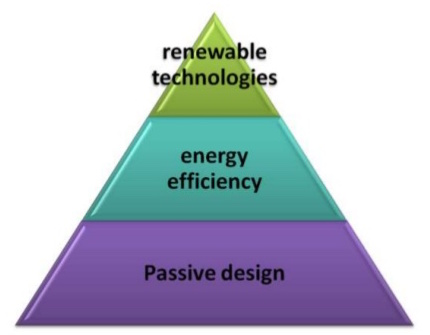
\includegraphics[width=10cm]{figures/Hierarchy.jpg}
	\rule{\textwidth}{0.5pt} % use line???
	\caption{The sustainable design hierarchy \citep{Dougherty:online}.}
	\label{fig_hierarchy}
\end{figure}


\begin{figure}[htbp]
	\centering
	
\includegraphics[width=\textwidth]{figures/SustainabilityAward.png}
	\rule{\textwidth}{0.5pt} % use line???
	\caption{First prize for sustainability awarded to my group for our library design in \textit{Critical Architectural Studies} (course code: D19CX).}
	\label{fig_award}
\end{figure}

\hl{Other courses?}
\begin{itemize}
	\item Use of solar gain in pool house (\textit{first year collaborative project})?
	\item Contact factor in \textit{LAB CFD}?
	\item Learned in \textit{CAS}, applied again in \textit{y4 collab}: make design concept red thread...
\end{itemize}


%----------------------------------------------------------------------------------------
%	SECTION 2
%----------------------------------------------------------------------------------------

\section{Engineering Analysis (EA)} \label{EA}

\subsection*{EA1(i, b, m)}

Conducting laboratory experiments and modelling exercises in \textit{Energy Principles and Applications}, \textit{Design Software Applications}, \textit{Thermal Performance Studies} and \textit{Laboratory Project} further developed my skills in monitoring, interpreting and applying the results of analysis to bring about continuous improvement (EA1i).
\textit{Laboratory Project} went a step further and taught me the principles and process to engineering a better solution (EA1b and EA1m).
These principles were applied in an engineering project which aimed to optimise the design of a cooling coil.
\hl{Analysis of key engineering processes???}


\subsection*{EA2(i, -)}

A range of courses have developed my ability to understand and explain the performance of systems and components through the use of quantitative/ analytical methods and/ or modelling techniques:
\textit{Construction Technology 2},
\textit{Acoustics and Architectural Design},
\textit{Hydraulics and Hydrology A},
\textit{Energy Principles and Applications},
\textit{Thermal Performance Studies},
\textit{Laboratory Project},
and \textit{Design Project}.
For example, in \textit{Hydraulics and Hydrology A}, I learned how to use quantitative methods to distinguish laminar flows from turbulent flows.
And when we were studying thermofluids in \textit{Laboratory Project}, I used both CFD modelling and analytical methods to understand and describe the performance of a cooling coil in an air conditioning unit.

I have also applied quantitative/ analytical methods and/ or modelling techniques to classify and describe the performance of systems during my work placements at Arup and Sweco.
In particular, at Sweco I used a combination of the aforementioned methods and techniques to describe the performance of some buildings in terms of solar heat gain, energy consumption, thermal comfort in winter and summer, and daylighting.
The results of these analyses were then classified according to the criteria of \textit{Miljöbyggnad}, i.e. the Swedish environmental certification system for buildings: Gold, Silver, Bronze or Disapproved.


\subsection*{EA3(i, b, m)}

I have developed my ability to use the results of analysis and apply quantitative and computational methods to solve engineering problems and subsequently recommend or implement appropriate action in the following courses:
\textit{Laboratory Project},
\hl{...}
For example, a combination of calculations, CFD modelling and a physical laboratory experiment were used to optimise the design of a cooling coil in \textit{Laboratory Project}.
This was an iterative process of solving problems and implementing appropriate actions to come up with a better solution.


\subsection*{EA4(i, b, m)}

\hl{See notes on Notion print-out from 26 Oct 2018}


\subsection*{EA5m}

In addition to my work placements at Hoare Lea and Sunamp, courses that I have developed my ability to use fundamental knowledge to investigate new and emerging technologies are
\textit{Energy and Buildings},
\textit{Innovation in Construction Practice},
\textit{Design Project},
and \textit{Dissertation}.
My most extensive investigation must be of Sunamp's heat batteries, having written the information sheets for their UniQ product range.


\subsection*{EA6m}

\hl{The only example I can think of is when I tried to calculate the yield of tidal power.
This was an unfamiliar problem and I could only find information online on how to calculate yields from hydroelectric turbines (?).
Thus, I had to use a combination of the information I found, assumptions and my own fundamental mathematical skillset.
Still, I never showed my workings to anyone, so I can't be sure if they were correct.

Fan's physics/ mathematical exercises at start of TPS?}

\hl{See notes on Notion print-out from 26 Oct 2018}

%----------------------------------------------------------------------------------------
%	SECTION 3
%----------------------------------------------------------------------------------------

\section{Design (D)}

\subsection*{D1(i, -)}

Multiple courses have developed and contributed to my understanding and ability to evaluate business, customer and user needs:
\textit{Introduction to Design},
\textit{Introduction to the Environment},
\textit{Environment and Behaviour},
\textit{Critical Architectural Studies},
\textit{Electrical and Lighting Services for Buildings},
\textit{Procurement and Contracts},
\textit{Facilities Management Principles},
\textit{Inclusive and Safe Environments},
and \textit{Design Project}.
The concept of a good brief that reflects the business, customer and user needs has been emphasised throughout the AE programme.
I have been able to evaluate such needs through various assignments and in different contexts, such as technical aspects (air quality, lighting levels and fire safety), users with different kinds of disabilities, and public perception.
During my placement at Hoare Lea, I was able to evaluate the design brief of a mixed-use new-build for needs regarding fire safety in order to design the fire detection and alarm systems.

%Some of these courses considered more technical needs such as good air quality and lighting levels, which are dependent on the functions of spaces.
%In \textit{Procurement and Contracts} and \textit{Facilities Management Principles}, I learned about the different stakeholders involved in a project and their respective needs and interests.


\subsection*{D2(i, -)}

\hl{Investigating and defining problems...}


\subsection*{D3(-, b, m)}

Working with information that may be incomplete or uncertain is something that I have found difficult.
\textit{Design Project B}, \textit{Design Project} and \textit{Laboratory Project} are courses that particularly challenged me in this area and helped me develop the skill.
During these projects I learned to make assumptions and use iterative/ trial-and-error processes to come up with a satisfactory design solution.
This was done, for example, for the sizing of pipes in the design projects.
\hl{However, I do not think I have ever gone as far as to quantify the effect of incomplete or uncertain information on a design and to use research to mitigate the deficiencies.}

\hl{See notes on Notion print-out from 26 Oct 2018}


\subsection*{D4(i, -)}

All design projects have developed my skills in creating design solutions that are fit for purpose:
\textit{1st year collaborative project},
\textit{Design Project A},
\textit{Design Project B},
\textit{Critical Architectural Studies},
\textit{Energy and Buildings},
and \textit{Design Project}, including the \textit{4th year collaborative project}.
\hl{Give examples?!
However, I cannot think of an example where the whole lifecycle was considered, especially disposal.}


\subsection*{D5(i, -)}

\hl{Plan and manage the design process, including cost drivers...
Design Project? I didn't do the timeline or costs...
I have always kind of avoided doing costing (CAS, collab projects (for appropriate reason)).}

\hl{See notes on Notion print-out from 26 Oct 2018}


\subsection*{D6}

\hl{Just in the context of design?}

Most of the assignments I have written and presentations I have given contributed to the development of my skill of communicating to technical or non-technical audiences.
Courses and work placements that have contributed to this skill development include:
\textit{Design Project A},
\textit{Construction Technology 2},
\textit{Hydraulics and Hydrology A},
\textit{Environment and Behaviour},
\textit{Design Project B},
\textit{Critical Architectural Studies},
\textit{Thermal Performance Studies},
\textit{Design Issues},
\textit{Facilities Management Principles},
\textit{Inclusive and Safe Environments},
\textit{Laboratory Project},
\textit{Design Project},
\textit{Dissertation},
\textit{Climate Change, Sustainability and Adaptation},
Sunamp,
Sweco?
Instances of communicating to non-technical audiences include my POSTnote assignment for \textit{Climate Change, Sustainability and Adaptation}, where I wrote about a technical topic to members of the UK parliament, and the Product Information Sheets that I created for Sunamp, which needed to convey the technical operation of their products in layman's terms.
Most laboratory reports I have written, e.g. for \textit{Laboratory Project}, were of a technical nature.


\subsection*{D7m}

I have been exposed to various UK building design and construction processes (especially the Royal Institute of British Architects (RIBA) Plan of Work 2013) and procurement routes during the following courses and work placements:
Arup,
\textit{Procurement and Contracts},
\textit{Facilities Management Principles},
Hoare Lea,
and
\textit{Dissertation}.
I have been able to contrast this knowledge with my (albeit limited) knowledge of Swedish building design and construction processes gained during my placement at Hultin \& Lundquist.
The thermofluids part of \textit{Laboratory Project} taught me about the methodology for optimising a design.
This knowledge has been complemented by information about specific \hl{parts/ scopes} of the design process, such as the briefing stage, site analysis, POEs and life cycle assessments, learned in
\textit{Construction Technology 1},
\textit{Introduction to Design},
\textit{Environment and Behaviour},
\textit{Facilities Management Principles},
and \textit{Sustainable and Intelligent Buildings}.
I have also delved into a study of BIM, a new way to approach collaborative building design which is the new ``Holy Grail" of design processes, during my \textit{Dissertation} and \textit{Innovation in Construction Practice}.
%UK vs Sweden: Arup, 
%HL, FMP, DST, P\&C vs H\&L
%BIM: DST, ICP
%Engineering optimisation: LAB
%From site analysis to POEs + LCA: Con tech 1, Intro to Design, Env and Beh, SIB
All of these courses and experiences have contributed to my wide knowledge and comprehensive understanding of design processes and methodologies.

I have developed my ability to apply and adapt this wide repository of knowledge and understanding of design processes and methodologies in the unfamiliar situations presented in \textit{Design Project} and \textit{Critical Architectural Studies}.
\hl{Elaborate?}
%Application in unfamiliar situations: DP, CAS


\subsection*{D8m}

\hl{New needs?}

\hl{See notes on Notion print-out from 26 Oct 2018}


%----------------------------------------------------------------------------------------
%	SECTION 4
%----------------------------------------------------------------------------------------

\section{Economic, Legal, Social, Ethical and Environmental Context (EL)}

\subsection*{EL1(-, m)}

I gained an understanding of the need for a high level of professional and ethical conduct in engineering and a knowledge of professional codes of conduct in \textit{Procurement and Contracts}.
I familiarised myself with CIBSE's and \hl{...} professional codes of conduct in an assignment where \hl{...}
This course and my ethical induction at Arup also taught me how ethical dilemmas can arise.
\hl{Elaborate?}


\subsection*{EL2}


\subsection*{EL3(i, -, m)}

Gantt chart? Learned about in ICP.
DP (but I didn't do this).
BIM process?

\hl{See notes on Notion print-out from 26 Oct 2018}


\subsection*{EL4(i, -)}

According to the oft-quoted Brundtland report, sustainable development is an approach to progress which meets the needs of the present generation without compromising the ability of future generations to meet their own needs.
\hl{Can't think of examples. Also, ability to apply quantitative techniques???}



\subsection*{EL5(-, m)}

The following courses increased my awareness of legal requirements governing engineering activities including \hl{health and safety (H\&S)}, liability issues, contracts and accessibility:
\textit{Design Issues},
\textit{Procurement and Contracts},
and \textit{Inclusive and Safe Environments}.
In particular, in \textit{Design Issues} I learned about the various UK regulations surrounding H\&S, including the Health and Safety at Work Act 1974 and the Construction (Design and Management) Regulations 2015, a.k.a. the CDM Regulations.
The CDM Regulations emphasise that H\&S need to be considered, not just on site, but throughout the planning and design stages also.
The designers, for example, have a responsibility to assess and eliminate or mitigate the H\&S risks associated with their design, whether that is during the construction or operation of the building.
Furthermore, this course broadened my awareness of legal requirements outside of the UK.
I learned about the H\&S regulations in France, the lack of building regulations in Guyana, and the ambitious building regulations with regards to sustainability in Singapore.
\hl{Is that a good demonstration of my knowledge?}

I have also applied my knowledge of legal requirements in a project for \textit{Inclusive and Safe Environments} and during my placements at Hoare Lea and Sweco.
At Hoare Lea I produced \hl{RIBA} Stage 3 layouts of fire detection and alarm installations for a new-build.
These were made to comply with standards such as \textit{BS 5839-6:2013 Fire detection and fire alarm systems for buildings - Part 6: Code of practice for the design, installation, commissioning and maintenance of fire detection and fire alarm systems in domestic premises}.
For instance, the standard stated the different radiuses that smoke detectors and heat detectors cover; I had to thus place the detectors on the plan layouts accordingly.


\subsection*{EL6(i, -, m)}

Many courses and a couple of my placements increased my awareness of risk issues.
I learned about risk issues related to H\&S at Sunamp and in
\textit{Electrical and Lighting Services for Buildings},
\textit{Design Issues},
\textit{Inclusive and Safe Environments},
and
\textit{Laboratory Project}.
In \textit{Electrical and Lighting Services for Buildings}, for example, I learned about the importance of earthing to give \hl{overflow?} electricity an alternative path to run through which is not a person (thus electrocuting them).
I learned about environmental risk issues in
\textit{Construction Technology 1},
\textit{Introduction to the Environment},
\textit{Thermal Performance Studies},
\textit{Sustainable and Intelligent Buildings},
\textit{Climate Change, Sustainability and Adaptation},
and
\textit{Water Supply and Drainage for Buildings}.
Throughout these courses I have learned about the impact of buildings and building systems on the environment, e.g. harmful refrigerants in air conditioners, embodied carbon in building materials, and the emissions from vehicles that people use to travel to buildings.
Lastly, I learned about \hl{commercial risk (?)} in \textit{Innovation in Construction Practice}, more specifically the risk of innovation in construction projects.
\hl{Elaborate?}

I learned about the techniques of risk assessment and risk management in depth in \textit{Design Issues} and have carried out H\&S risk assessments in \textit{Facilities Management Principles}, \textit{Laboratory Project} and during my placement at Arup.
\hl{Attach LAB risk assessments?}
Generally, one first needs to identify the risks and then assess them in terms of severity and likelihood.
Afterwards, one tries to eliminate the risks (the worst first), and if that is not possible, mitigate them.


\subsection*{EL7m}

For business success, I have only gained an understanding of how innovation is a key driver in \textit{Innovation in Construction Practice} and \hl{how technology (?) plays a role in business success through the study of Fordist and post-Fordist consumerism/ manufacturing?} in \textit{Sustainable and Intelligent Buildings}.
\hl{Look up ICP and SIB notes + elaborate.}

Due to the nature of my academic programme, I have not learned as much about the key drivers for business success as I have for successful construction projects in the following courses:
\textit{Introduction to Design},
\textit{Procurement and Contracts},
\textit{Facilities Management Principles},
\hl{and more?}
However, there are two ways that this knowledge can translate to business.
Firstly, a construction project is often a means for a business to grow or improve (\hl{this is known as a secondary business case? see FM notes}).
Therefore, a successful construction project can lead to a successful business.
Secondly, the principles behind a successful construction project should also be able to be applied to businesses.
For example, after the construction sector was pointed out in the 1990s for repeatedly delivering projects that were of poor quality, overtime and over-budget, the sector has made significant efforts to improve its performance and improve client satisfaction.
Such efforts have resulted in changing the workflow so that more planning is done at the start of a project, when making changes is more flexible and less costly (\hl{get figure from ICP?}).
This includes developing more descriptive briefs, which set out the client's needs and how the construction project should be run.
\hl{I imagine this could translate in such a way to business... think!}


%----------------------------------------------------------------------------------------
%	SECTION 5
%----------------------------------------------------------------------------------------

\section{Engineering Practice (P)}


\subsection*{P1(i, -)}

Throughout the programme, I have gained a knowledge and understanding of some contexts in which my Architectural Engineering knowledge can be applied.
The following list in which I describe such contexts is not exhaustive.

\begin{enumerate}
	\item The collaborative design projects in years \hl{1/2} and 4,
	\textit{Building Services Technology},
	\textit{Introduction to the Environment},
	\textit{Design Project A},
	\textit{Design Project B},
	\textit{Electrical and Lighting Services for Buildings},
	\textit{Critical Architectural Studies},
	\textit{Design Project},  
	and my placements at Arup and Hoare Lea
	provided me with the practical experience of applying my AE knowledge in the context of a team designing a building and/ or its services, in which I was responsible for the building services, the building's internal environment and the occupants' comfort levels.
	
	\item Through
	\textit{Acoustics and Architectural Design},
	\textit{Environment and Behaviour},
	\textit{Energy Principles and Applications},
	\textit{Energy and Buildings},
	\textit{Thermal Performance Studies},
	\textit{Design Issues},
	\textit{Facilities Management Principles},
	\textit{Laboratory Project},
	\textit{Sustainable and Intelligent Buildings},
	\textit{Climate Change, Sustainability and Adaptation},
	\textit{Water Supply and Drainage for Buildings},
	my work in the environmental certification of existing buildings at Sweco,
	and
	my encounter with a specialist in Performance at Hoare Lea,
	Design Issues,
	I have also learned that my AE knowledge is applicable in the operation and management of buildings and building services (a.k.a. facilities management) to, for example, improve the occupants' comfort levels, optimise performance or increase resilience to future impacts of climate change.
	
	\item Through the work I did at Sunamp as well as my encounter with a technical author at Hoare Lea, I understand that engineering knowledge is important in the composition of technical documents (e.g. specifications, operation and maintenance manuals) and even marketing material for technical products, which may need to explain engineering processes in layman's terms.
	
	\item My \textit{Dissertation} in particular taught me that engineering knowledge is necessary for the development of industry standards and codes of practice, such as the series of Publicly Available Specifications (PAS) 1192 which standardise the requirements for achieving BIM Level 2.
	
	\item Throughout my \textit{Dissertation} and \textit{Climate Change, Sustainability and Adaptation}, I have also come to understand that my engineering knowledge can be used for research, the development of new technologies or processes, and to influence policies. \hl{Repeated DST and CCSA. Could even include Sunamp. Maybe this example is one too many...}
\end{enumerate}


\subsection*{P2(i, -, m)}

I have gained a knowledge of the characteristics of, an understanding of and an ability to use a range of computer-based tools, building services products, and engineering processes:
\begin{itemize}
    \item P2i 
     
     In \textit{Environment and Behaviour}, \textit{Laboratory Project} and \textit{Dissertation}, I developed an ability to use the statistics software tool SPSS (Statistical Package for the Social Science).
     The course \textit{Statistics for Science} provided me with a foundation to understand the data in the inputs and outputs of this software.
    
    \item P2i and P2
    
    In \textit{Design Software Applications} and \textit{Laboratory Project}, I gained an in-depth understanding of the characteristics of steady-state and dynamic building modelling and energy analysis software programmes, notably iSBEM, SAP, IES, and CFD.
    As these courses only provided an introduction to these software programmes, I have not mastered my ability to use them.
    This was demonstrated during my attempt to model my \textit{Design Project} building in IES; my building model overheated due to variation and temperature profiles that I had incorrectly set up, amongst other things.
    
    During the \textit{Design Project} and my placements at Hultin \& Lundquist Arkitekter and Sunamp, I gained an understanding of and an ability to use Autocad.
    Likewise, I learned to use Revit during the \textit{Design Project} and my placements at Arup and Hoare Lea.
    Although my ability to use these Autodesk products (i.e. Autocad and Revit) is limited, I have learned quite a bit about their characteristics.
    In \textit{Dissertation} and \textit{Innovation in Construction Practice}, I learned about the prominent use of these products in the UK construction industry and how their proprietary characteristics can lead to problems of interoperability.
    
    Regarding engineering processes, I have learned extensively about the BIM process in Dissertation and Innovation in Construction Practice.
    I have also learned the characteristics of and practised the optimisation process of an engineering design in \textit{Laboratory Project} (see EA3(i, b, m) in Section \ref{EA} for more detail \hl{is this the correct reference where I expand on the optimisation of cooling coil?}).
    
    \item P2m
    
    I have gathered an extensive knowledge and understanding of a wide range of building services products (e.g. heat pumps, heat batteries, photovoltaic panels) and building materials (e.g. phase-change materials, Ziegel blocks, steel)
    throughout many of my construction-based courses, i.e. 
    \textit{Construction Technology 1},
    \textit{Building Services Technology},
    \textit{Design Project A},
    \textit{Construction Technology 2},
    \textit{Acoustics and Architectural Design},
    \textit{Design Project B},
    \textit{Critical Architectural Studies},
    \textit{Electrical and Lighting Services for Buildings},
    \textit{Design Software Applications},
    \textit{Energy and Buildings},
    \textit{Thermal Performance Studies},
    \textit{Design Project},
    \textit{Laboratory Project},
    \textit{Sustainable and Intelligent Buildings},
    \textit{Innovation in Construction Practice},
    and \textit{Water Supply and Drainage for Buildings},
    and my placements at Sunamp, Hoare Lea and Arup
\end{itemize}


%Building materials: insulation, steel, wood, Ziegel blocks, glass, PCMs etc.

%Building services products: ACs, HPs, PV, AHUs, Sunamp, windcatchers






%----------------------------------------------------------------------------------------
%	SECTION 6
%----------------------------------------------------------------------------------------

\section{Additional General Skills (G)}
\chapter{Personal Reflection} % Main chapter title

\label{Chapter4} % Change X to a consecutive number; for referencing this chapter elsewhere, use \ref{ChapterX4}

\lhead{Chapter 4. \emph{Personal Reflection}} % Change X to a consecutive number; this is for the header on each page - perhaps a shortened title



%----------------------------------------------------------------------------------------
%	SECTION X
%----------------------------------------------------------------------------------------

\section{Professionalism}

A professional is someone that:
\begin{itemize}
    \item Applies their body of knowledge with rigorous standards of skill, care and diligence,
    \item Seeks continuously to maintain up to date \& to improve knowledge \& skills in themselves and others,
    \item Is entirely trustworthy, ethical and acts with integrity.
    \item Fulfils an overriding duty to society/mankind and thereafter the client 
    \item Treats all people fairly \& with respect 
\end{itemize}

Points to discuss:
\begin{itemize}
    \item log (and then asked for it, glad on reflection for my initiative/ proactiveness);
    \item needing to be opportunistic rather than strategic to see Sandy (stats on number of meetings...);
    \item Applies their body of knowledge with rigorous standards of skill, care and diligence;
    \item personal project and carrying out a personal programme of work (G3);
    \item compilation of work produced.
\end{itemize}


\subsection{Log Keeping}

During my first placement at Hultin \& Lundquist Arkitekter in 2013, I was asked to keep a timesheet which I was to submit on a monthly basis.
As I was getting paid an hourly rate, my salary was calculated from that timesheet.

When I started my placement at Arup in 2016, I knew from reading my contract that the company expected me to produce and submit a report about my placement by the end of it.
I therefore kept a daily diary where I jotted down notes about the work I had done and the things I had learned in addition to recording the hours I worked.
This not only facilitated the writing of the report, but also helped me monitor the progress of my tasks/ assignments and strengthen my knowledge acquisition.

From these experiences, I developed a habit of keeping a log at my following placements for my own benefit but also in case my employers required me to submit a timesheet.
Sometimes this was the case (e.g. at Hoare Lea and Sunamp), and other times it was not (e.g. at Sweco).
A month into my placement at Sunamp, for example, I was asked to submit a timesheet.
On reflection, I am glad for my proactivity in keeping a log at Sunamp since they did not inform me on the timesheet requirement at the start of my placement.

\st{
When I started my placement at Arup in 2016, I knew from reading my contract that the company expected me to produce and submit a report about my placement by the end of it.
I therefore kept a daily diary where I jotted down notes about the work I had done and the things I had learned in addition to recording the hours I worked.
This not only facilitated the writing of the report, but also helped me monitor the progress of my tasks/ assignments and strengthen my knowledge acquisition.
Due to the multiple benefits of logging, I continued to do so/ made it a habit at my following placements, even though I was not required to submit a report, except for the Industrial Project.

When I started my summer placement at Sunamp in 2018, I decided to keep a more systematic log to facilitate the writing of the Industrial Project report in the autumn.
}





%----------------------------------------------------------------------------------------
%	SECTION X
%----------------------------------------------------------------------------------------
\newpage
\section{Academic Performance}



%----------------------------------------------------------------------------------------
%	SECTION X
%----------------------------------------------------------------------------------------

\section{Perfectionism vs. Time Management}



%----------------------------------------------------------------------------------------
%	SECTION X
%----------------------------------------------------------------------------------------

\section{Future Learning and Career Aspirations}
\chapter{Conclusion} % Main chapter title

\label{Chapter5} % Change X to a consecutive number; for referencing this chapter elsewhere, use \ref{Chapter5}

\lhead{Chapter 5. \emph{Conclusion}} % Change X to a consecutive number; this is for the header on each page - perhaps a shortened title


%----------------------------------------------------------------------------------------
%	THESIS CONTENT - APPENDICES
%----------------------------------------------------------------------------------------

\addtocontents{toc}{\vspace{2em}} % Add a gap in the Contents, for aesthetics

\appendix % Cue to tell LaTeX that the following 'chapters' are Appendices

% Include the appendices of the thesis as separate files from the Appendices folder
% Uncomment the lines as you write the Appendices

% Appendix Template

\chapter{The UniQ Overview Sheet} % Main appendix title

\label{AppendixA} % Change X to a consecutive letter; for referencing this appendix elsewhere, use \ref{AppendixX}

\lhead{Appendix A. \emph{The UniQ Overview Sheet}} % Change X to a consecutive letter; this is for the header on each page - perhaps a shortened title

Write your Appendix content here.

%\includepdf[pages=-]{Appendices/}
% Appendix Template

\chapter{The UniQ Product Selection Quiz} % Main appendix title

\label{AppendixB:quiz} % Change X to a consecutive letter; for referencing this appendix elsewhere, use \ref{AppendixX}

\lhead{Appendix B. \emph{The UniQ Product Selection Quiz}} % Change X to a consecutive letter; this is for the header on each page - perhaps a shortened title

The final UniQ Product Selection Quiz is on the following page.

%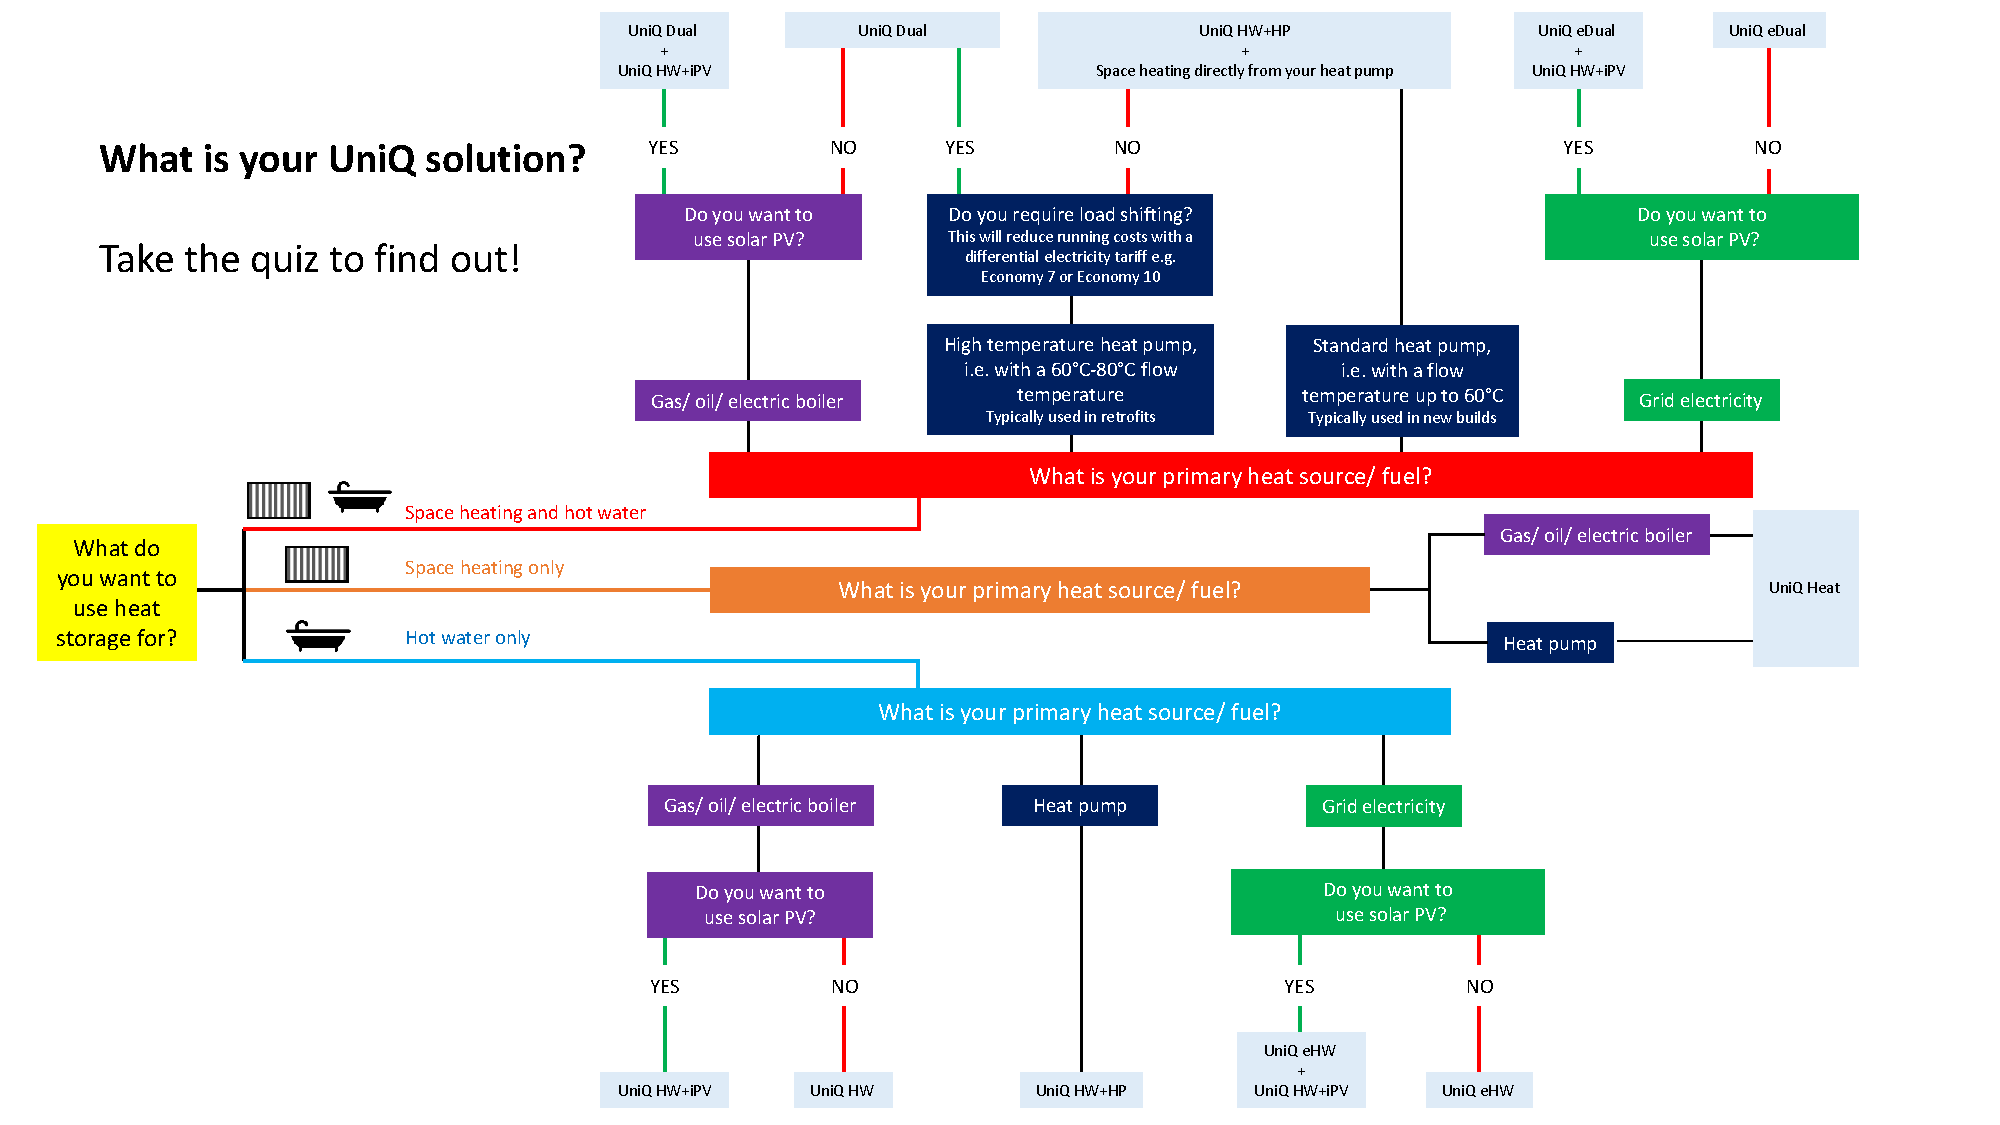
\includepdf[pages=-,height=\textheight]{Appendices/final_quiz.pdf}

%\begin{figure}
%	\centering
%	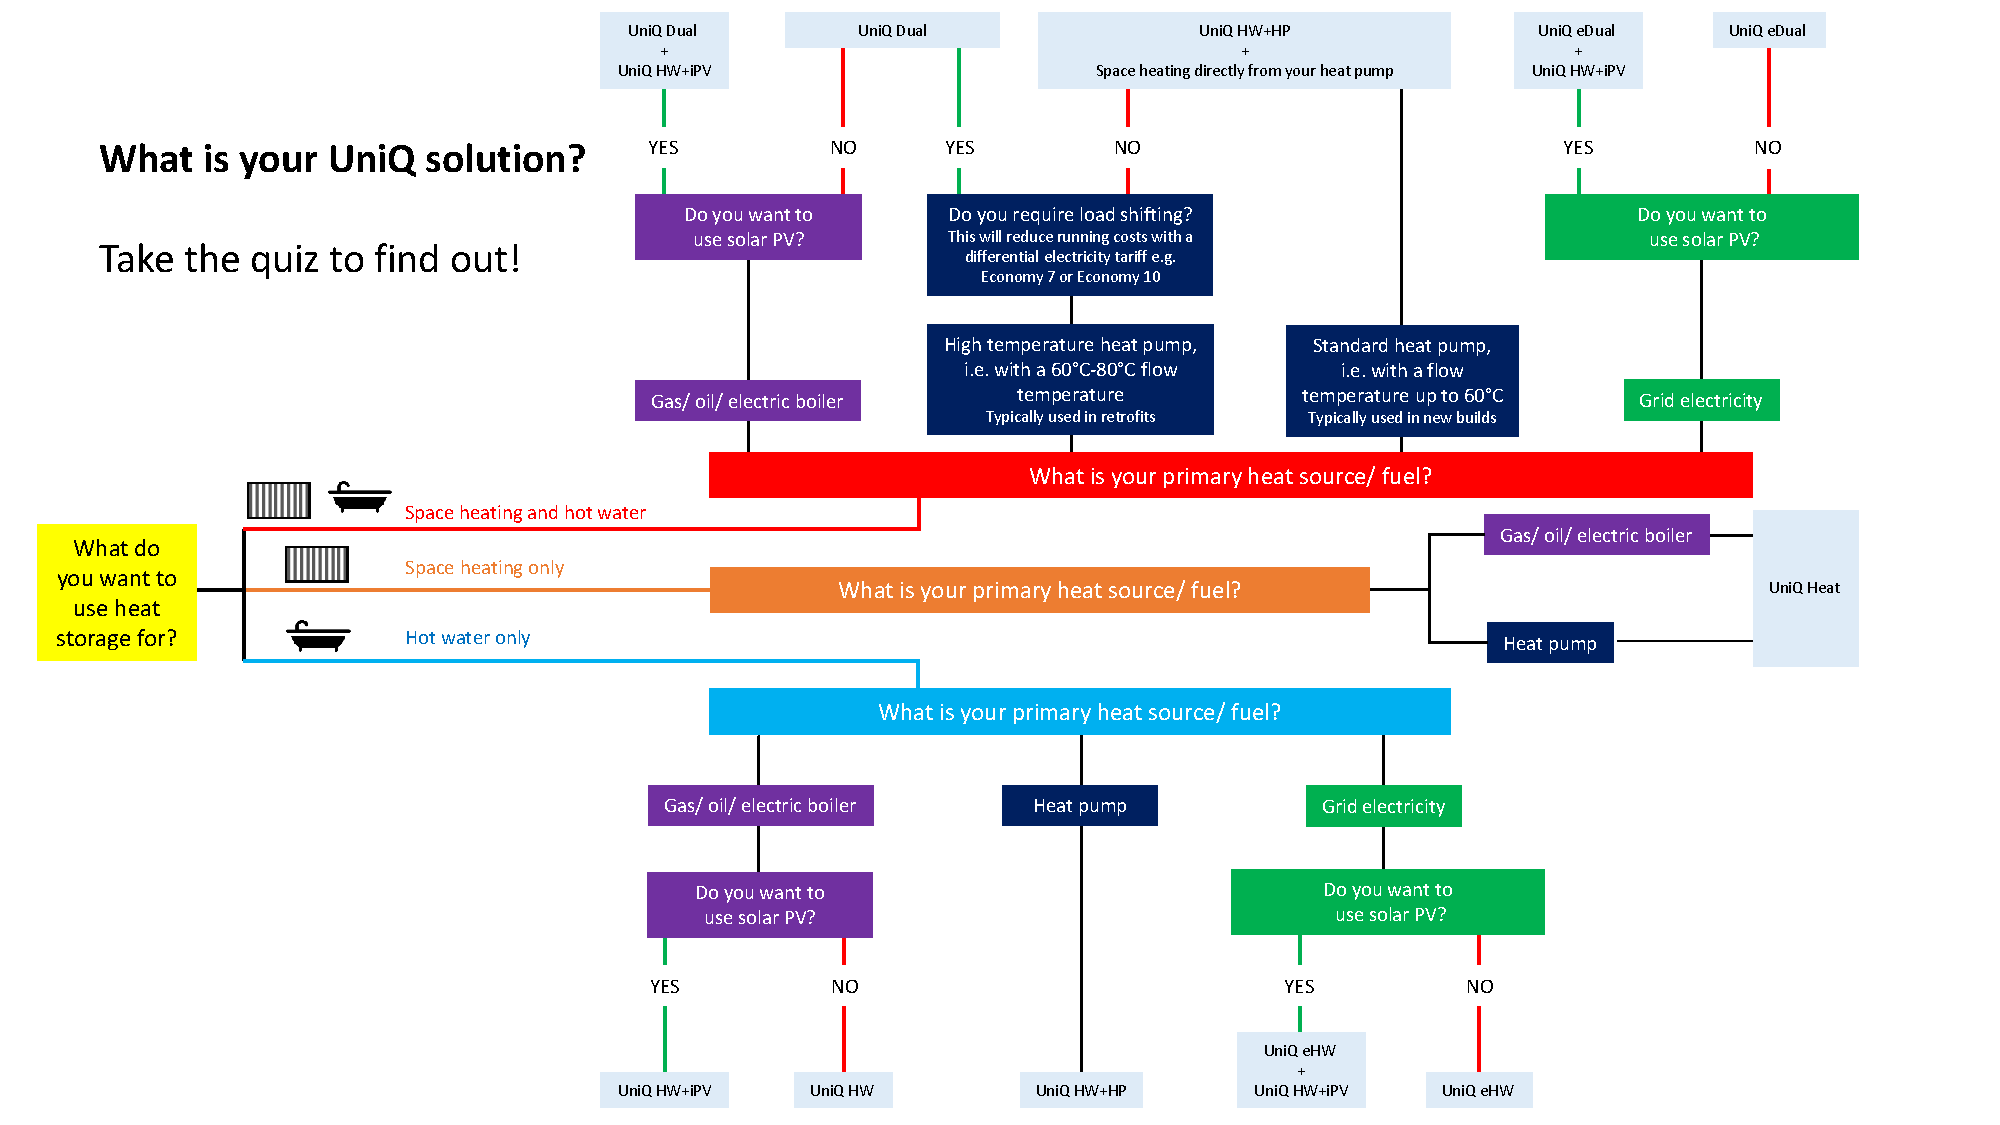
\includegraphics[height=\textheight]{Appendices/final_quiz.pdf}
%\end{figure}

\begin{sidewaysfigure}
    \centering
	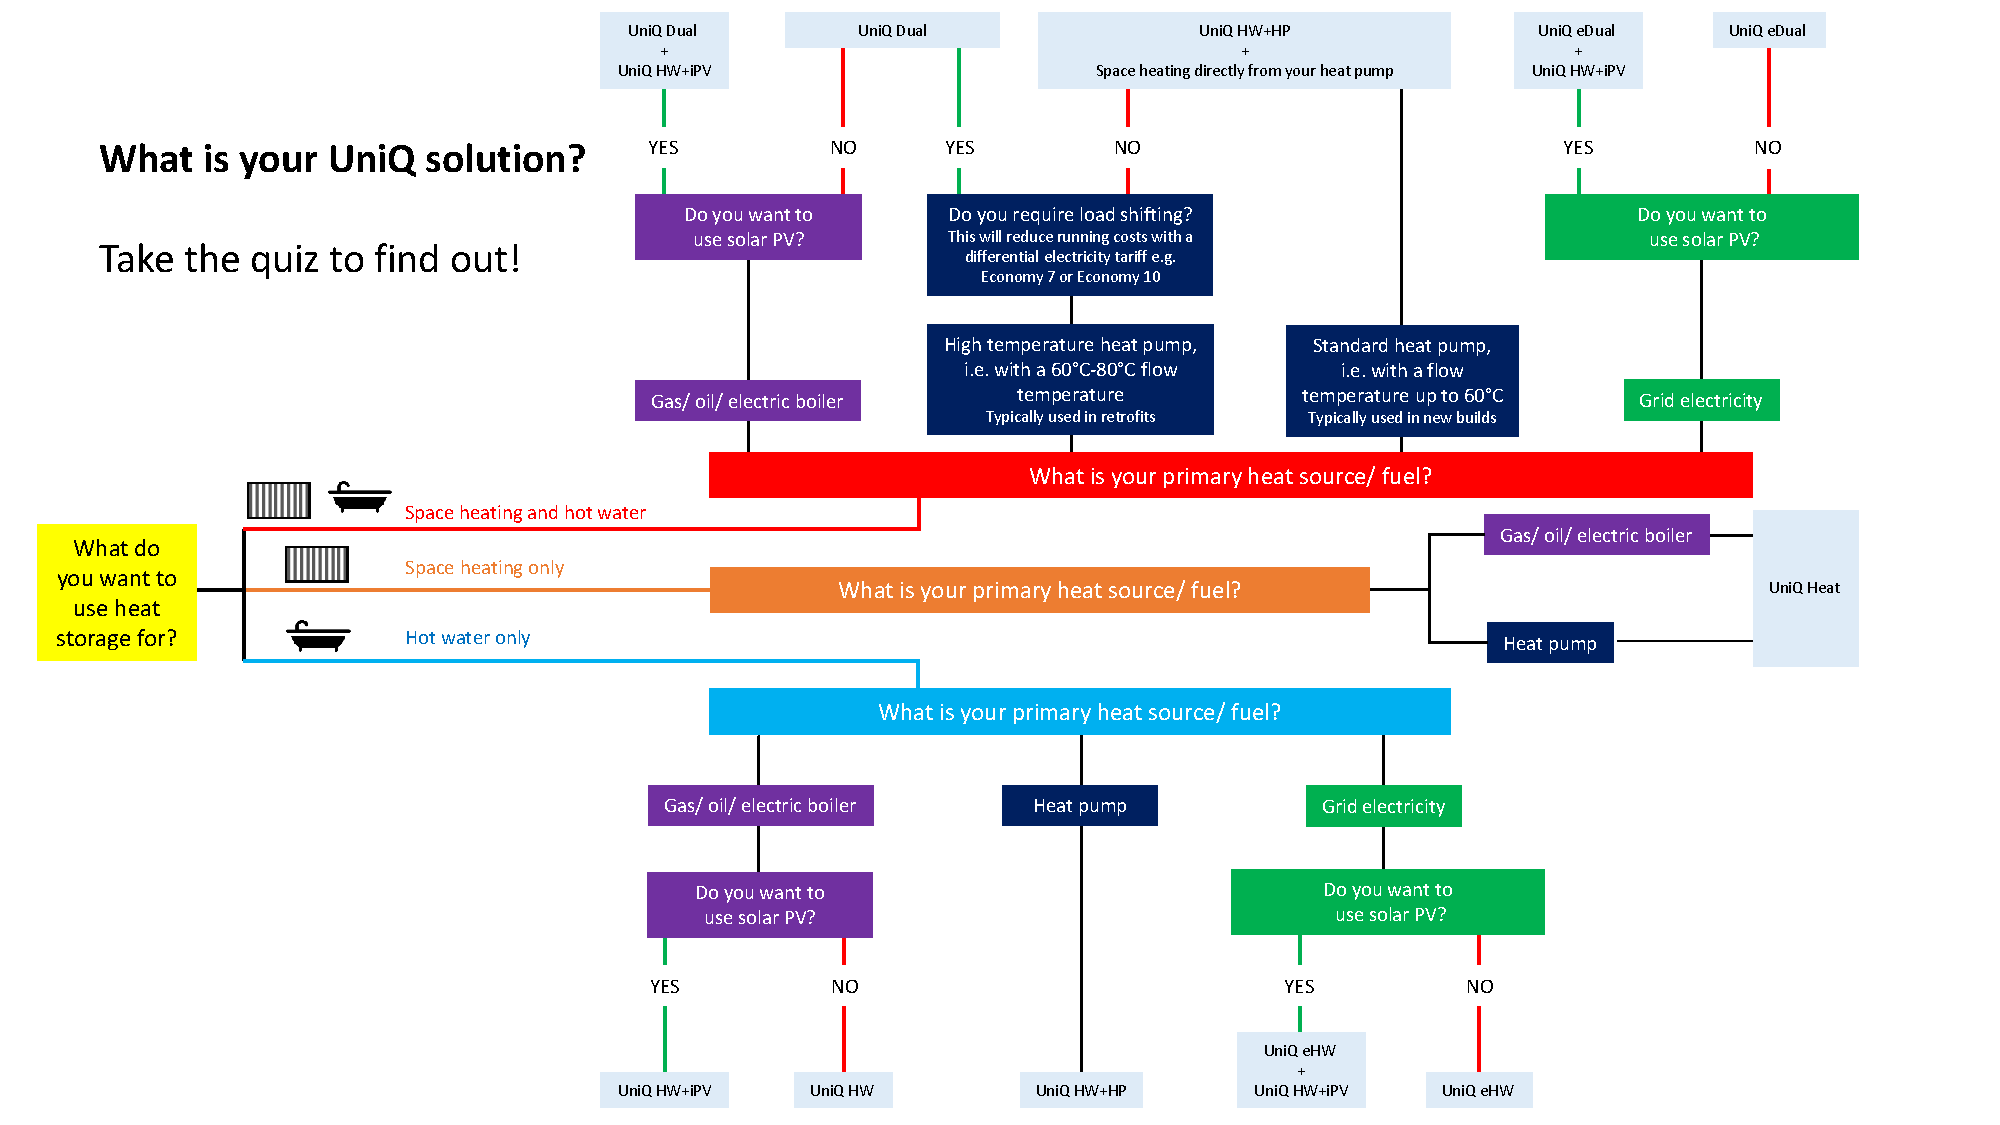
\includegraphics[width=\textwidth]{Appendices/final_quiz.pdf}
\end{sidewaysfigure}
% Appendix Template

\chapter{The UniQ Product Information Sheets} % Main appendix title

\label{AppendixC} % Change X to a consecutive letter; for referencing this appendix elsewhere, use \ref{AppendixX}

\lhead{Appendix C. \emph{The UniQ Product Information Sheets}} % Change X to a consecutive letter; this is for the header on each page - perhaps a shortened title

The UniQ PIS drafts that I left with Sunamp start on the following page.

\begin{itemize}
    \item \textcolor{red}{Texts in red} express my uncertainties in their expression or phrasing; these may require amending by Sunamp. This includes all the taglines.
    \item I have expressed other uncertainties as comments.
\end{itemize}

%\begin{sidewaysfigure}
%    \centering
%	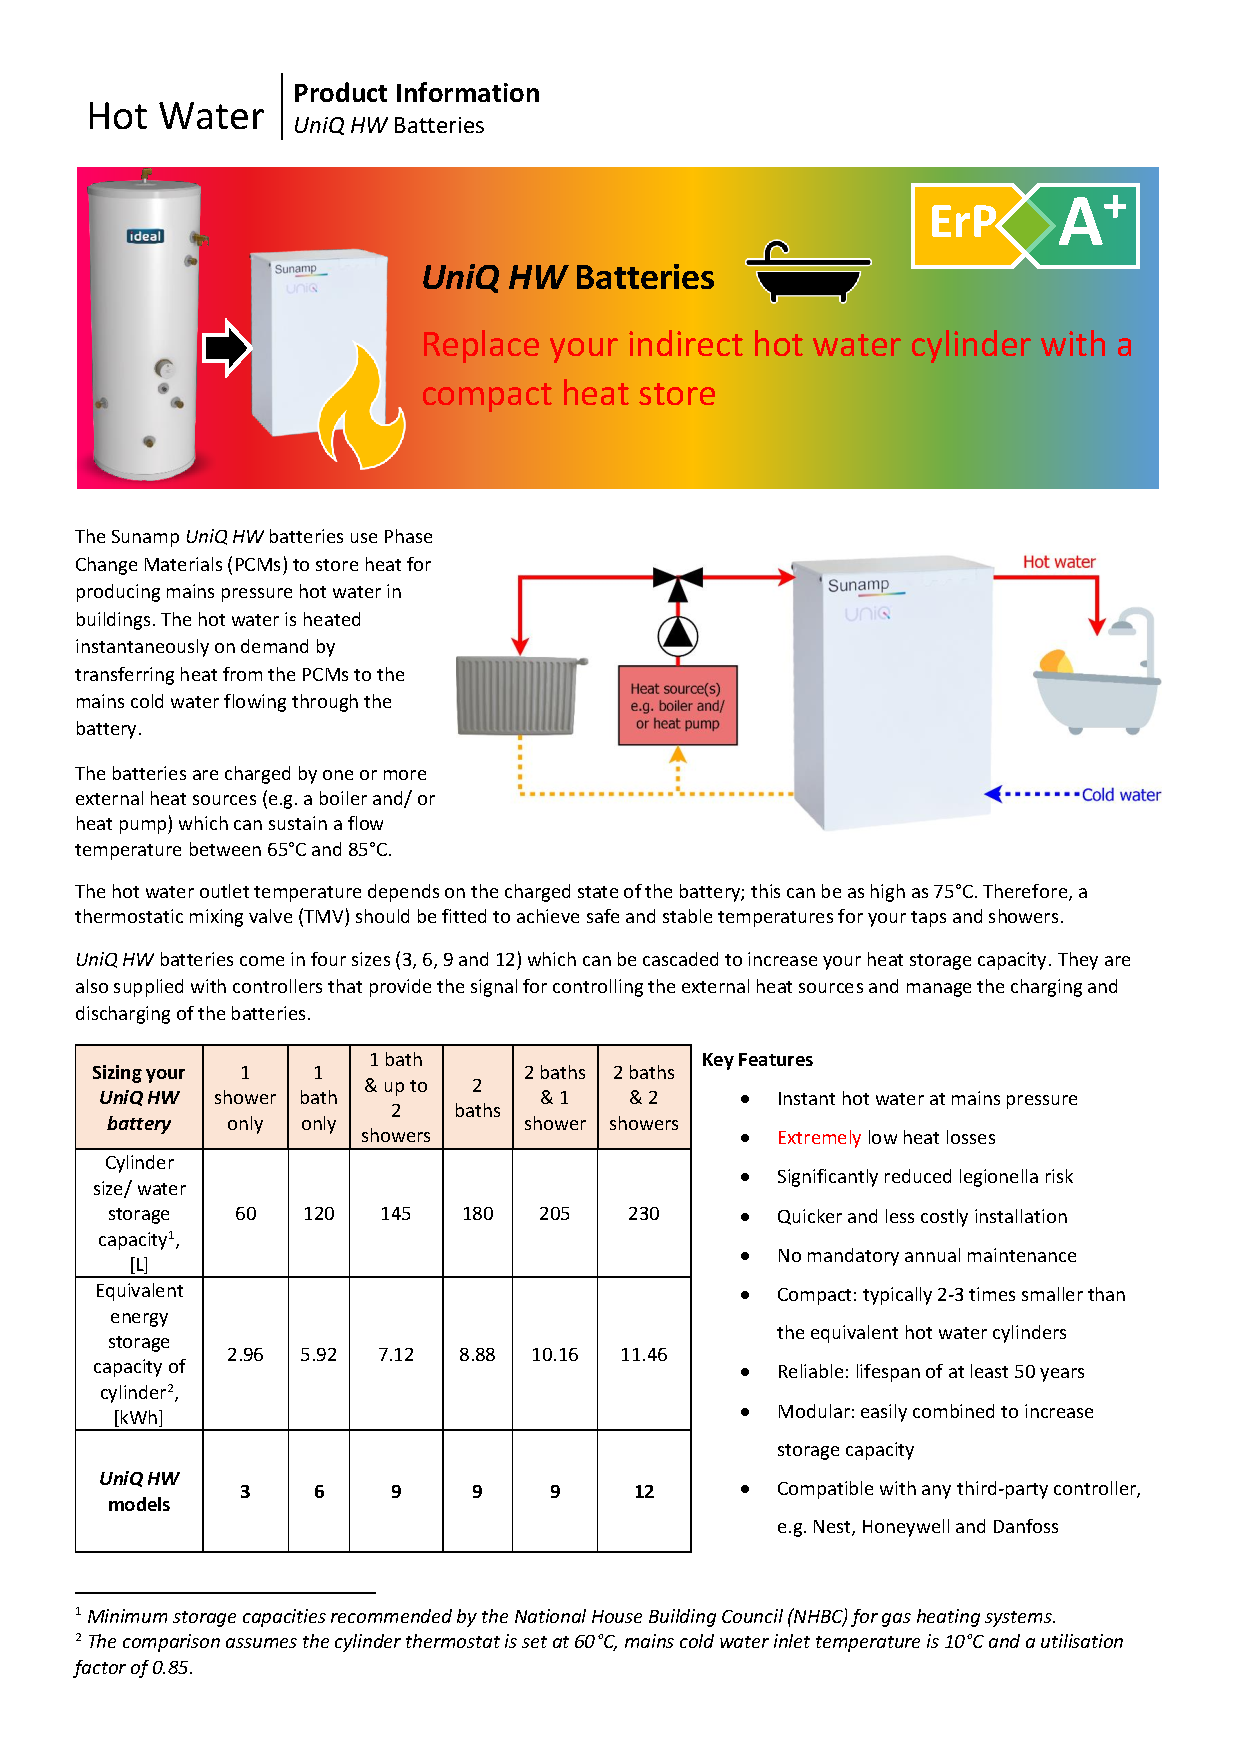
\includegraphics[width=\textwidth]{Appendices/1_PIS_HW.pdf}
%\end{sidewaysfigure}

% DECIDE HOW TO INCLUDE PDFS

% OPTION 1
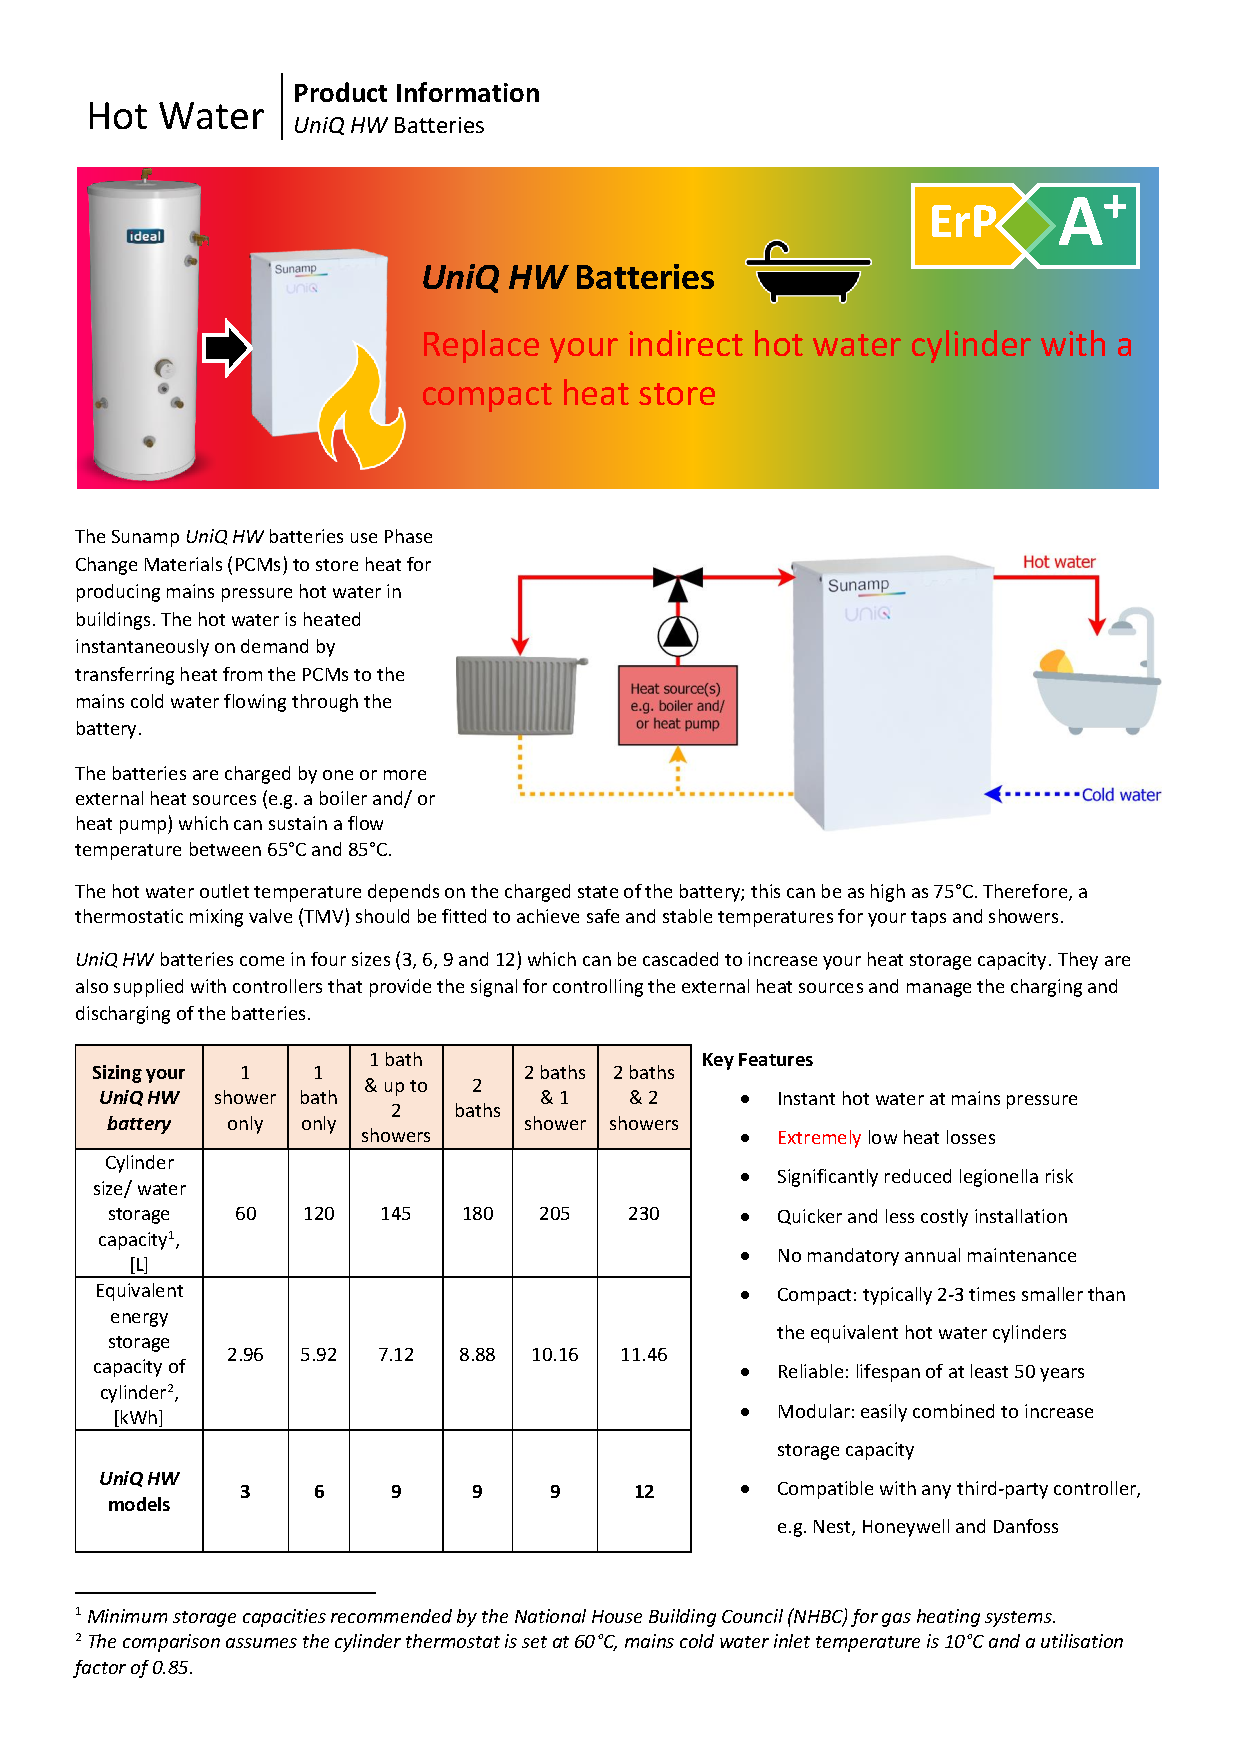
\includepdf[pages=-, offset=2cm -2cm]{Appendices/1_PIS_HW.pdf}

% OPTION 2
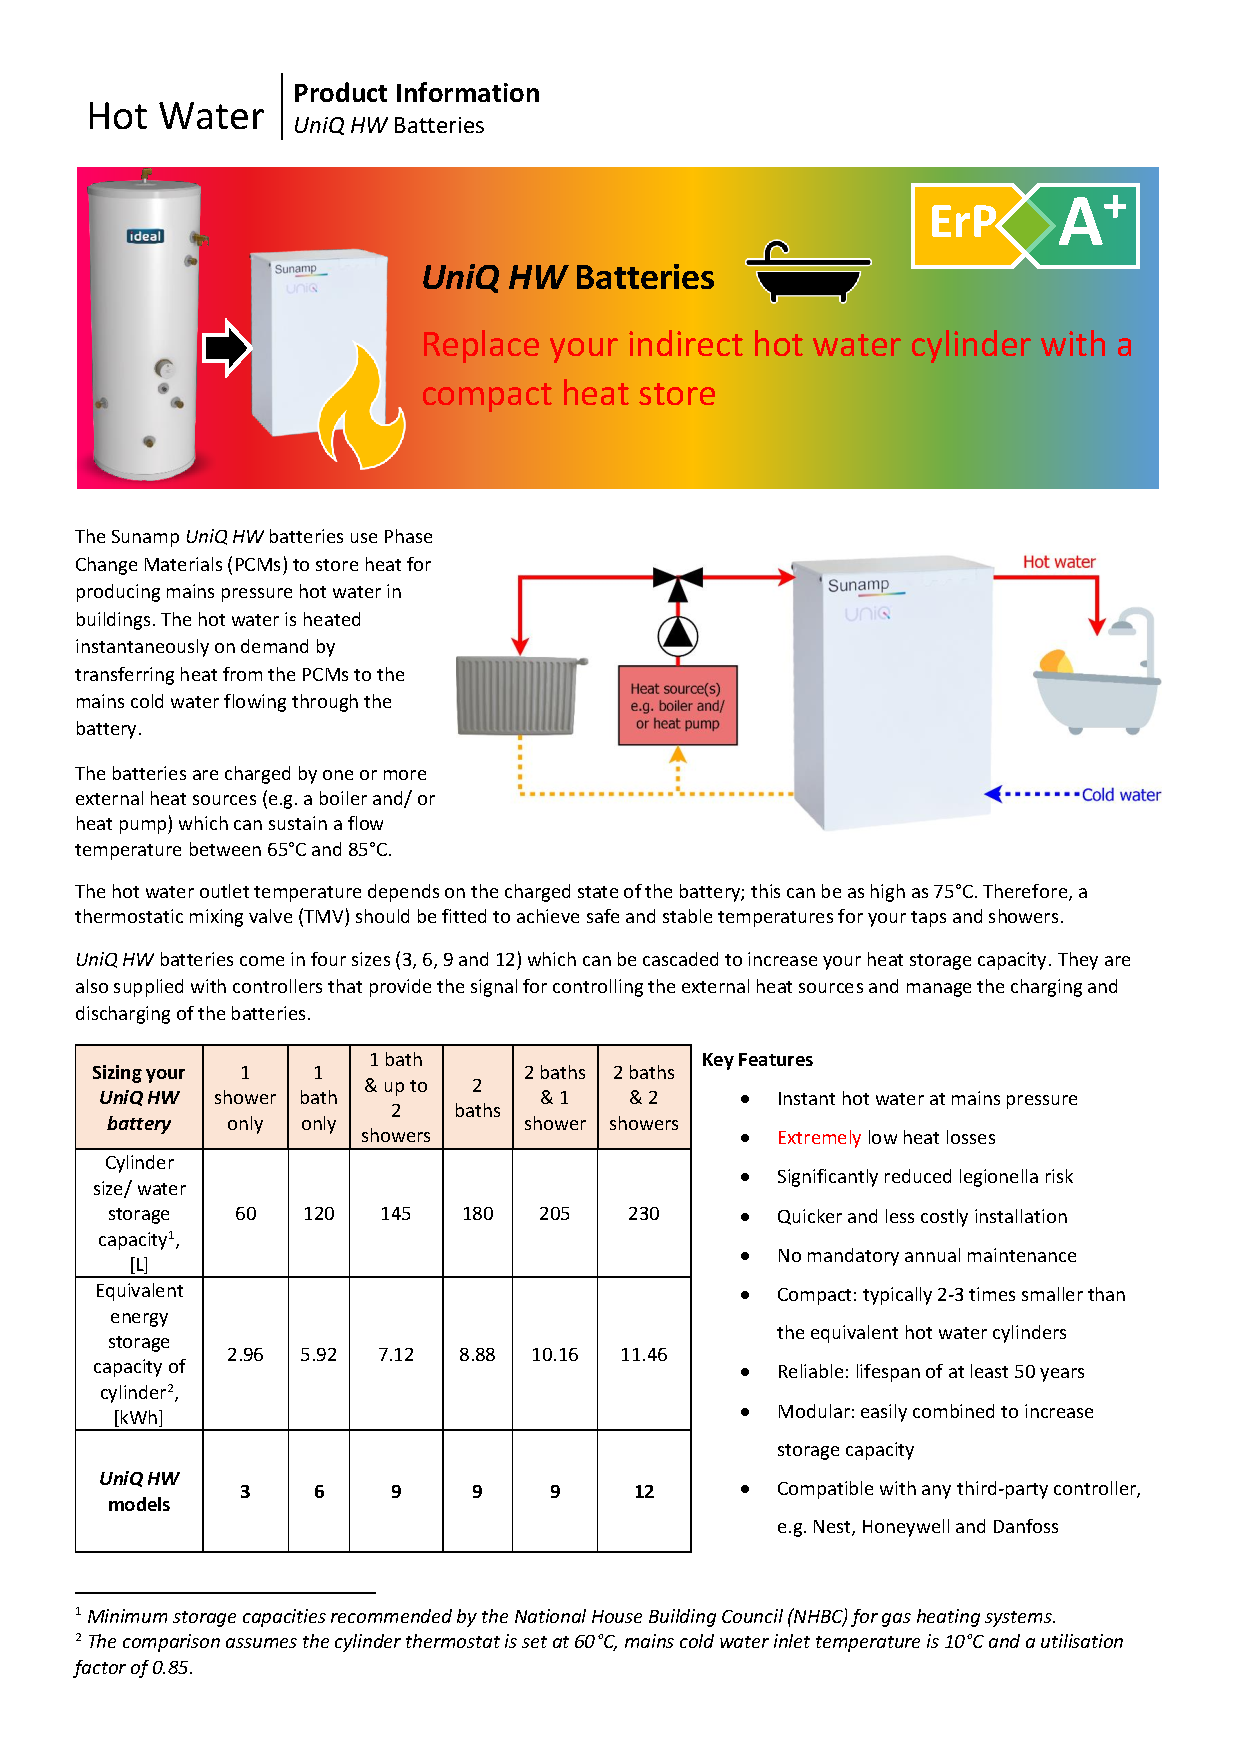
\includepdf[pages=-,height=\textheight, offset=2cm -2cm]{Appendices/1_PIS_HW.pdf}

% OPTION 3
\begin{figure}
	\centering
	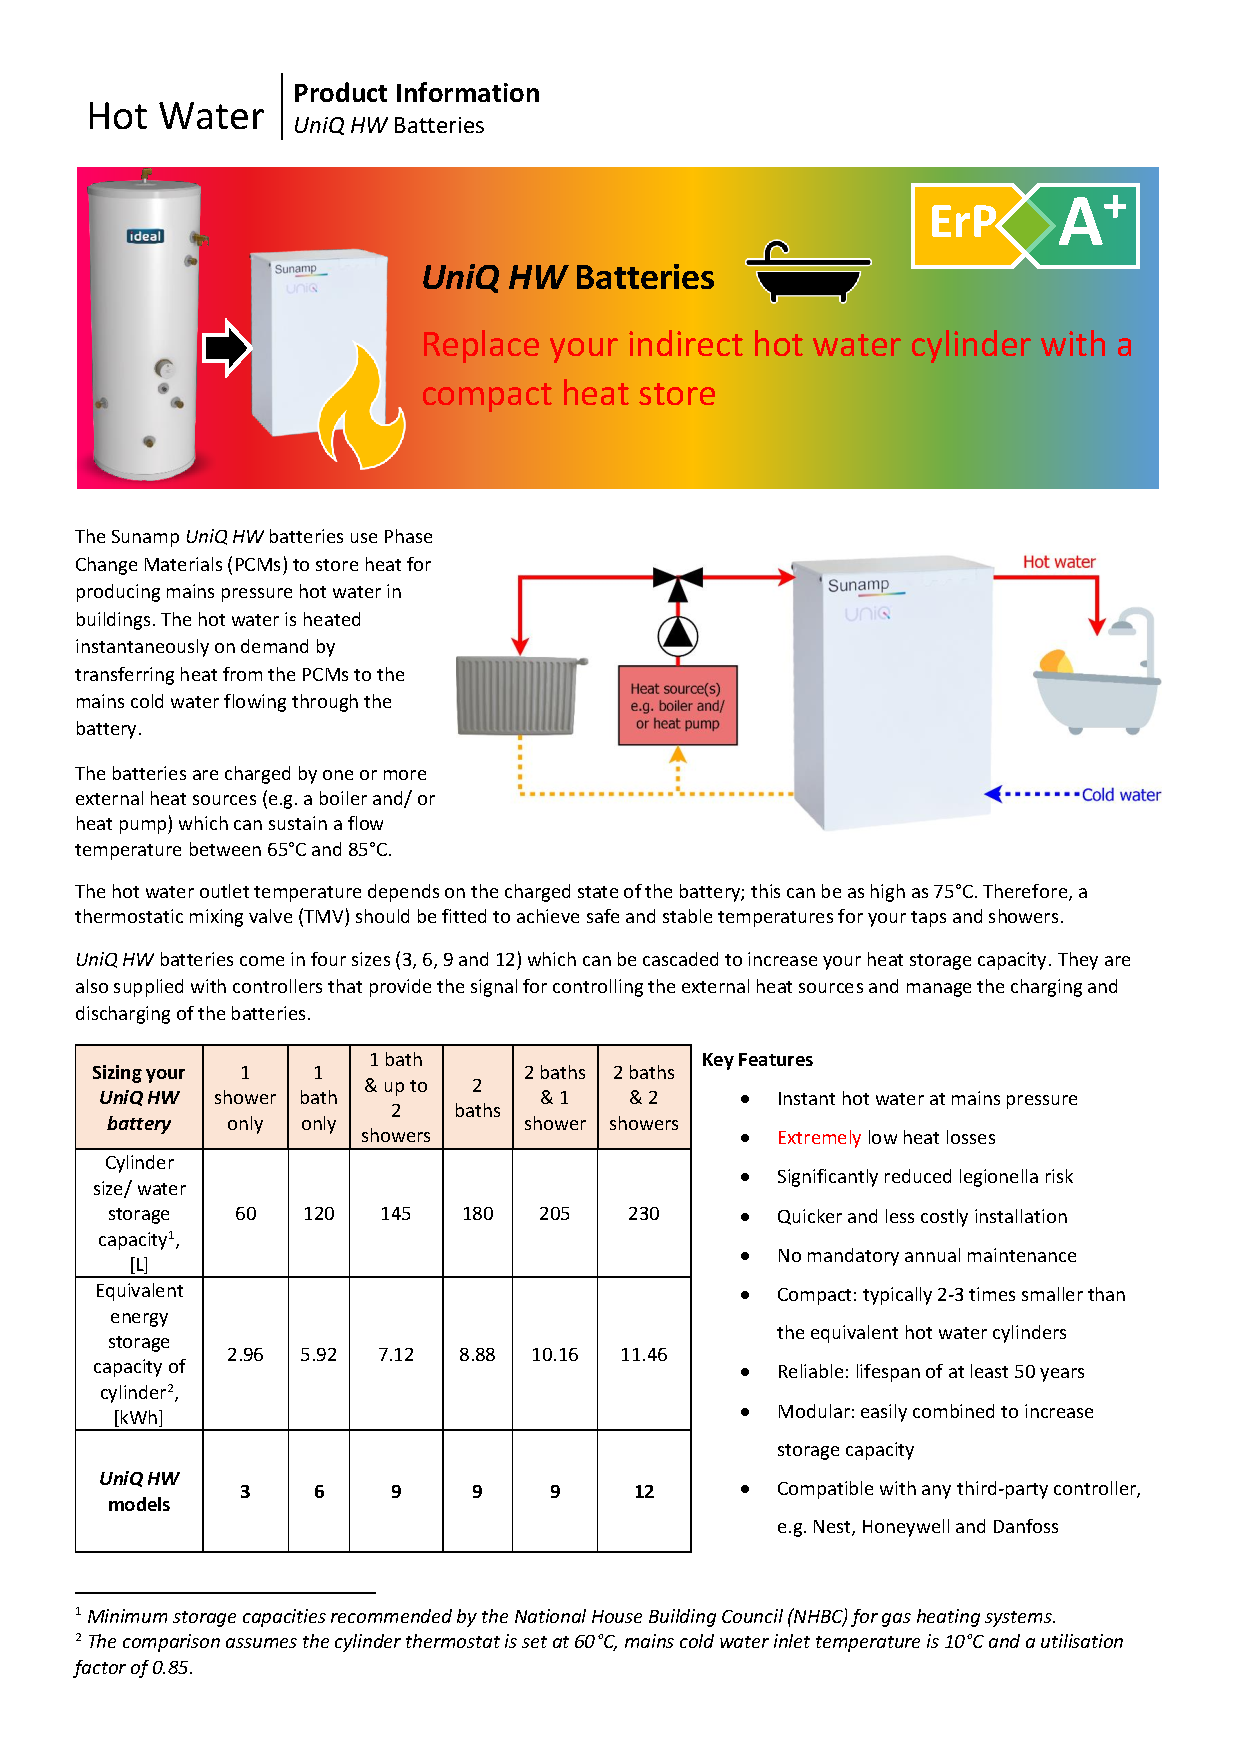
\includegraphics[height=\textheight]{Appendices/1_PIS_HW.pdf}
\end{figure}


\addtocontents{toc}{\vspace{2em}} % Add a gap in the Contents, for aesthetics

\backmatter

%----------------------------------------------------------------------------------------
%	BIBLIOGRAPHY
%----------------------------------------------------------------------------------------

\label{Bibliography}

\lhead{\emph{References}} % Change the page header to say "Bibliography"

\bibliographystyle{apalike} % Use the "apalike" BibTeX style for formatting the Bibliography

\bibliography{Bibliography} % The references (bibliography) information are stored in the file named "Bibliography.bib"

\end{document}